% =====================================================================
% Revised version (v4) after the project-idea review.
% Built from DCOP_Idea_Review_v3.tex. Needs arxiv.sty and references.bib from the
% Overleaf project (not in this folder). Figures and tables are generated (from the repo root) by
%   python3 -m vmgm.figures vmgm_results/full paper
% which writes them straight into paper/figures/ and paper/tables/.
%
% Lines marked  % TODO(team)  need a decision or a check before submission.
% Every number in the text comes from vmgm_results/full/summary.md.
% =====================================================================
\documentclass{article}
\usepackage{arxiv}
\usepackage[utf8]{inputenc}
\usepackage[T1]{fontenc}
\usepackage{hyperref}
\usepackage{url}
\usepackage{booktabs}
\usepackage{amsfonts,amsmath,amssymb,amsthm}
\usepackage{microtype}
\usepackage{natbib}
\usepackage{xcolor}
\usepackage{tabularx}
\usepackage{array}
\usepackage{enumitem}
\usepackage{float}
\usepackage{graphicx}
\usepackage{cleveref}
\usepackage{multicol}
\usepackage{tikz}
\usepackage{titlesec}
\titlespacing*{\section}{0pt}{7pt plus 2pt}{4pt}
\usetikzlibrary{positioning,calc}

\setlist{itemsep=0pt,topsep=1pt,parsep=0pt,partopsep=0pt,leftmargin=1.2em}
\setlength{\textfloatsep}{6pt plus 2pt minus 2pt}
\setlength{\floatsep}{5pt plus 2pt minus 2pt}
\setlength{\intextsep}{5pt plus 2pt minus 2pt}
\setlength{\abovedisplayskip}{3pt}\setlength{\belowdisplayskip}{3pt}
\setlength{\abovedisplayshortskip}{2pt}\setlength{\belowdisplayshortskip}{2pt}
\setlength{\abovecaptionskip}{2pt}\setlength{\belowcaptionskip}{2pt}

\theoremstyle{definition}
\newtheorem{definition}{Definition}
\newtheorem{result}{Result}

\newcommand{\1}{\mathbf{1}}
\newcommand{\gmax}{g_{\max}}

\title{Who Is Gaming the Timetable? Catching Dishonest Departments\\ in Distributed Exam Scheduling}
\date{}
\usepackage{authblk}
\renewcommand\Authfont{\bfseries}
\setlength{\affilsep}{0.3em}
\author{Beli Dedhia}
\author{Khushi Garg}
\author{Ananya Patel}
\author{Poojan Soni}
\affil{Indian Institute of Technology Gandhinagar}
\renewcommand{\headeright}{Revised after review}
\renewcommand{\undertitle}{Multi-Agent Systems: Project (revised after the idea review)}
\renewcommand{\shorttitle}{Who Is Gaming the Timetable?}
\hypersetup{colorlinks=true,linkcolor=blue!55!black,citecolor=blue!55!black,urlcolor=blue!55!black}

\begin{document}
\maketitle
\vspace{-2.2em}
\begin{abstract}
In MGM, a standard distributed algorithm, the department that \emph{announces} the biggest improvement moves first, so a liar can grab turns or stop progress. In exam timetabling, the clash and back-to-back part of each improvement can be recomputed by anyone from public data; only the preference part is private, and it lies on a fixed scale $0$ to $\gmax$. Checking one announcement at a time misses repeated small lies; checking a department's history of claims catches every contradiction; lies that never contradict themselves cannot be caught from public data. With the history check and quarantine of caught departments we prove three \emph{separate} guarantees: the student cost a liar's own moves add is below $\gmax$ per exam; the run always finishes; and the final cost exceeds the starting cost by at most $2\gmax$ per dishonest exam. No bound relative to honest MGM's result is possible, so that is measured: with up to 6 of 12 departments dishonest, every blocker and churner was flagged, every run finished, and the final cost was $1.10$--$1.71$ times honest MGM's, mostly the cost of quarantine itself.
\end{abstract}

%=====================================================================
\section{Introduction}
%=====================================================================
\textbf{Problem.} Exam timetabling puts each exam in a slot so that no student has two exams at once (a \emph{clash}) and few students have exams in consecutive slots on the same day (\emph{back-to-back}) \citep{carter1996}. Departments also prefer some slots. The information is split: the registrar knows how many students each pair of exams shares, and each department knows its own preferences. In a distributed version \citep{meisels2003}, departments keep preferences private and set their own exams' slots; no central solver sees everyone's preferences, and only a public \emph{notice board} is trusted. This is a Distributed Constraint Optimization Problem (DCOP) \citep{yokoo1998,fioretto2018}. The agents are departments, and some may be dishonest (course Directions~A and~B).

\textbf{Why dishonesty matters.} Local search is the usual choice when a problem is too large for exact DCOP methods \citep{fioretto2018}. In MGM \citep{maheswaran2004mgm}, each round every department works out the best single change it could make and posts how much that change would lower the total cost (its \emph{gain}). Among neighbours, only the largest posted gain moves. MGM trusts these numbers: a huge fake gain always wins and can freeze neighbours, and moving an exam back and forth can stop the search from finishing.

\textbf{Key observation.} In a general DCOP, a department that is not part of a cost function cannot recompute that cost, so posted gains are taken on trust. In exam timetabling, clash and back-to-back costs depend only on the shared-student counts and the timetable, which are on the board, so \emph{every} department can recompute that part of a gain. Only the preference part is private, and it can change by at most $\gmax$.

\textbf{Research question.} \emph{How much can dishonest departments harm MGM in distributed exam timetabling, and how much of that harm can be detected and limited by checking posted gains against public data only, without payments or repeating work on several agents?}

\textbf{Example} ($W_h=10$ per student per clash, $W_s=2$ per student per back-to-back pair, $\gmax=50$). EE's exam $e_1$ clashes with CSE's $c_1$ (3 shared students, cost $10\times3=30$) and is back-to-back with $m_1$ (2 shared students, cost $2\times2=4$). Moving $e_1$ to slot~3 removes both, so the public gain is $V=34$, which anyone can recompute. EE also likes slot~3 better by $10$ points, so its private gain is $P=10$. The honest claim is $34+10=44$ and passes. A claim of $100$ implies a private gain of $66>50$, which is impossible, so it is flagged. Now suppose EE moves $e_1$ from slot~3 to~4 claiming slot~4 is better by $40$, and later from~4 back to~3 claiming slot~3 is better by $40$. Each claim alone is within $50$, but together they cannot both be true. Only a check of the \emph{history} of claims catches this.

\textbf{What is new.} Earlier work on untrustworthy DCOP agents uses payments or repeated computation, for other kinds of algorithms (\Cref{sec:prelim}). To our knowledge (based on our search), checking the announcements of local search has not been studied. From the public/private split we build two checks and show which lies they catch and which no check can catch. We then separate three guarantees that are easy to conflate: the damage a liar does \emph{directly} through its own moves (bounded), whether the run \emph{finishes} (guaranteed with quarantine), and the \emph{total} cost of the final timetable (bounded relative to the start, but not relative to honest MGM, so measured). Experiments with up to half the departments dishonest test each one. MGM and DSA are existing algorithms.

%=====================================================================
\section{Preliminaries}
\label{sec:prelim}
%=====================================================================
\begin{definition}[DCOP]
Agents each set their own variables (finite value sets) and talk only to agents they share a cost function with; the goal is to minimise the total cost \citep{fioretto2018}.
\end{definition}

\textbf{Local search.} In DSA \citep{zhang2005}, an agent that can improve its cost makes the change with a fixed probability $p_{\text{DSA}}$. In MGM \citep{maheswaran2004mgm}, only an agent whose posted gain beats all its neighbours' moves (ties broken by a fixed rule); with honest agents the total cost never increases.

\textbf{Related work.} M-DPOP \citep{petcu2008mdpop} uses payments (VCG) so that running the algorithm honestly is each agent's best choice; we use no payments. \citet{noshiro2026} study agents that may behave arbitrarily badly (Byzantine faults) in DCOPs, prove a limit on how many such agents can be tolerated, and make the Max-Sum algorithm robust by repeating each computation on several agents (replication). Replication needs several agents that know the same cost, but only one department knows its preferences, so we aim for detection and limited damage instead. Privacy-preserving DCOP algorithms hide costs and assignments \citep{tassa2019,goldklang2025}; we instead publish them so gains can be checked.

\textbf{Notation.} Departments $1,\dots,N$; $E_i$ the exams of department $i$; slots $1,\dots,S$, each on a day; timetable $\sigma$ ($\sigma_e$ is exam $e$'s slot); $n_{ef}$ students shared by exams $e,f$ ($\bar n$: average over pairs with $n_{ef}>0$); neighbours of $i$ share students with it; $g_e(a)\in\{0,\dots,\gmax\}$ is the cost of putting $e$ in slot $a$; selfishness $\lambda_i\ge1$; $k$ dishonest departments, whose exams form $E_L$; a move $\mu=(e,a')$ puts exam $e$ into slot $a'$.

%=====================================================================
\section{Problem Formulation}
\label{sec:form}
%=====================================================================
\textbf{Costs.} For each pair of exams sharing students,
$f_{ef}(a,b)=W_h n_{ef}\1[a=b]+W_s n_{ef}\1[|a-b|=1 \text{ and same day}]$. Then
\begin{equation}
H(\sigma)=\textstyle\sum_{\{e,f\}}f_{ef}(\sigma_e,\sigma_f),\qquad G(\sigma)=\sum_e g_e(\sigma_e),\qquad F=G+H \ \text{(to minimise)}.
\label{eq:cost}
\end{equation}
$H$ is the student cost and $G$ the preference cost. Each department's \emph{burden} $B_i=\sum_{e\in E_i}[g_e+\frac12\sum_f f_{ef}]$ splits every shared cost half-half, so $\sum_iB_i=F$.

\textbf{Assumptions.} A1: $n_{ef}$, $W_h$, $W_s$, days, allowed slots and $\gmax$ are published before the run. A2: the board shows the timetable and every announcement; posts cannot be forged, and all departments post in the same rounds. A3: each $g_e$ is private, takes integer values in $\{0,\dots,\gmax\}$, and does not change during a run. A4: a move changes one exam. A5: the board applies only the posted move of a department that won its turn.

\textbf{Gains.} For a move $\mu=(e,a')$ by department $i$, with current slot $a=\sigma_e$:
\begin{equation}
V=\textstyle\sum_{f}\big[f_{ef}(a,\sigma_f)-f_{ef}(a',\sigma_f)\big]\ \text{(public)},\qquad P=g_e(a)-g_e(a')\ \text{(private, } |P|\le\gmax),\qquad \Delta=V+P.
\label{eq:gain}
\end{equation}
$\Delta$ is the drop in total cost $F$. A selfish department cares about $J_i=\lambda_iG_i+H_i$ (its own preferences weighted by $\lambda_i$, plus all student costs touching its exams), whose gain is $U_i=V+\lambda_iP$. Each round, department $i$ posts a move $\hat\mu_i$ and a claimed gain $\hat\Gamma_i$. Anyone can compute $r_i=\hat\Gamma_i-V$, the private part the department is \emph{claiming}.

\begin{definition}[Truthful]
Post the move with the largest $\Delta$ and claim exactly $\Delta$ if it is positive; otherwise post ``no move'' and $0$. Then $r_i=P$.
\end{definition}

\textbf{Protocol.} A department moves only if its priority is positive and beats every neighbour's (in plain MGM, priority $=\hat\Gamma_i$). With honest departments, neighbours never move together, so $F$ strictly falls and MGM stops.

\textbf{Who can lie.} \emph{Honest} departments are truthful; \emph{selfish} ones try to lower their own $J_i$; \emph{malicious} ones try to raise $F$. A liar knows the public data, the board and its own $g$, but not others' $g$, and controls only its own posts. Any number $k$ of departments may lie, each independently. Liars working together (collusion), fake identities, tampering with public data and out-of-turn posts are out of scope; \Cref{sec:limits} explains which guarantees still hold under collusion. We treat the attacks in \Cref{tab:attacks} as a fixed threat model, as in security analysis, not as equilibrium play.

\begin{table}[!t]
\caption{Attacks and whether each check flags them (``if incons.'': once its claims contradict each other). The last two rows are new attacks built to stress the guarantees.}
\label{tab:attacks}
\centering\footnotesize
\setlength{\tabcolsep}{4pt}\begin{tabularx}{\linewidth}{@{}>{\raggedright\arraybackslash}p{0.75cm}>{\raggedright\arraybackslash}p{4.1cm}X>{\raggedright\arraybackslash}p{2.0cm}>{\raggedright\arraybackslash}p{2.0cm}@{}}
\toprule
ID & Attack (goal) & What it posts & One-post check & History check \\
\midrule
T1a/b & Exaggerate (selfish): naive/consistent & own $U_i$ / truthful for a fake $\tilde g$ & if $|\lambda P|>\gmax$ / never & if incons. / never \\
T2a/b & Inflate (selfish): huge/in scale & $U_i+10^6$ / $V+\gmax$ & yes / never & yes / if incons. \\
T3a/b & Block/churn (malicious) & $10^6$ always / best-$V$ move, claim $V+\gmax$ & yes / never & yes / if incons. \\
T4 & Sabotage (malicious) & harmful move ($-\gmax<V<0$), claim $V+\gmax$ & never & if incons. \\
T5 & Consistent sabotage (malicious) & most harmful move that keeps its history consistent, largest consistent claim & never & never \\
T6 & Delayed contradiction & T5 for 20 rounds, then T3a & from round 20 & from round 20 \\
\bottomrule
\end{tabularx}
\end{table}

\textbf{Research questions.} Let $\rho=F(\text{final})/F(\text{final, honest MGM})$ from the same start. \textbf{RQ1:} how much do attacks raise $\rho$, and do they stop the run from finishing? \textbf{RQ2:} with $k$ dishonest departments, how many does each check flag, does the run finish, how much damage is done directly and in total, and who pays for it? \textbf{RQ3:} how much can an undetectable liar gain, depending on $\lambda$ and $\kappa=\gmax/(W_s\bar n)$ (preference size vs.\ back-to-back cost)? \textbf{RQ4:} how does damage depend on problem size, overlap and the liar's number of neighbours?

%=====================================================================
\section{V-MGM and What It Guarantees}
\label{sec:sol}
%=====================================================================
\begin{result}[One-post check is safe]
\label{res:one}
Under A1--A4, a truthful post is either ``no move'' with claim $0$, or has $|r_i|\le\gmax$. \emph{Proof:} $r_i=P=g_e(a)-g_e(a')$, and both values lie in $\{0,\dots,\gmax\}$.
\end{result}
So we cap priority at $\min\{\hat\Gamma_i,\,V+\gmax\}$ ($0$ for ``no move'') and flag a post if $|r_i|>\gmax$. Honest posts are never flagged or changed, but a lie within the scale is never flagged, however often it is repeated.

\begin{result}[History check catches every contradiction]
\label{res:hist}
Each claim about exam $e$ says ``slot $a_t$ costs me $r_t$ more than slot $a'_t$''. The claims are \emph{consistent} if some preference $\tilde g$ on the scale satisfies $\tilde g(a_t)-\tilde g(a'_t)=r_t$ for all of them. Keep a running score per slot: start at $0$ for the first slot, and after each move set score$(a')=$ score$(a)-r$.\footnote{Recording every consistent claim, including claims whose move does not run, gave identical results in all runs.} % TODO(team): pick 'posted' or 'executed' (code: protocol['record']) and keep this footnote only if needed.
Flag if a slot visited again gets a different score, or if the highest and lowest scores differ by more than $\gmax$. This flags exactly the inconsistent histories, and never a truthful one. \emph{Why:} if the scores agree and fit within $\gmax$, then $\tilde g=$ score $-$ lowest score explains every claim.
\end{result}

\begin{result}[Consistent lies cannot be detected]
\label{res:undet}
A department that posts truthfully for a fake preference $\tilde g$ on the scale (T1b) produces exactly the board of an honest department whose real preference is $\tilde g$, so no public check can detect it.
\end{result}

\textbf{V-MGM} is MGM with capped priority, one of the two checks, and a response to flagged departments: \emph{cap only} (keep the capped priority) or \emph{quarantine} (priority capped at $V$, so only moves that lower the student cost can run) (\Cref{fig:flow}). Every department runs the checks itself on public data, so no honest department can be framed. Our main method is the history check with quarantine; the results below say exactly what it guarantees, and \Cref{tab:guarantees} summarises them.

\begin{figure}[!t]
\centering
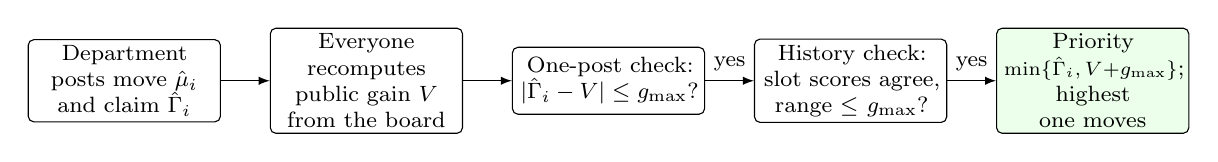
\begin{tikzpicture}[font=\footnotesize, box/.style={draw, rounded corners=2pt, align=center, inner sep=3pt, text width=2.3cm, minimum height=0.85cm, inner sep=2pt}, >=latex]
\node[box] (a) {Department posts move $\hat\mu_i$ and claim $\hat\Gamma_i$};
\node[box, right=0.62cm of a] (b) {Everyone recomputes public gain $V$ from the board};
\node[box, right=0.62cm of b] (c) {One-post check: $|\hat\Gamma_i - V|\le\gmax$?};
\node[box, right=0.62cm of c] (d) {History check: slot scores agree, range $\le\gmax$?};
\node[box, right=0.62cm of d, fill=green!8] (e) {Priority\\ {\scriptsize$\min\{\hat\Gamma_i, V{+}\gmax\}$};\\ highest one moves};
\draw[->] (a) -- (b); \draw[->] (b) -- (c);
\draw[->] (c) -- node[above]{yes} (d); \draw[->] (d) -- node[above]{yes} (e);
\end{tikzpicture}
\caption{How V-MGM handles one post. A ``no'' at either check flags the department (cap only, or quarantine: priority capped at $V$). Honest posts always pass, so with honest departments V-MGM behaves exactly like MGM.}
\label{fig:flow}
\end{figure}

\begin{result}[Direct damage limit]
\label{res:bound}
With capped priority and the history check, the moves of an exam made while its owner is unflagged raise the student cost $H$ by less than $\gmax$ in total. With quarantine, this holds for the exam's moves over the whole run, so department $i$'s own moves add less than $|E_i|\,\gmax$ to $H$. \emph{Why:} a move runs only if its priority is positive, so $r_m>-V_m$. Adding up an exam's claimed private parts, the scores of the in-between slots cancel and the total is at most the score range, which is at most $\gmax$. After quarantine, every move has $V_m>0$.
\end{result}
Result~\ref{res:bound} is a bound on \emph{direct} damage only: the student cost added by the liar's own moves. It does not bound the total cost, which also depends on how honest departments react and on improvements that were blocked, and it does not hold with cap-only (a flagged department can keep adding cost). Results~\ref{res:term}--\ref{res:global} add the two missing guarantees; Result~\ref{res:neg} shows what cannot be guaranteed.

\begin{result}[Termination]
\label{res:term}
With the history check and quarantine, every run finishes, for any number $k$ of dishonest departments.
\emph{Proof.} For each dishonest department $j$, fix once a preference $\tilde g_j$ on the scale that explains every claim $j$ made before it was flagged (it exists by Result~\ref{res:hist}; if $j$ is never flagged, take its whole history). Let
$\Phi=H+\sum_{i\text{ honest}}G_i+\sum_{j\text{ dishonest, unflagged}}\tilde G_j$, where $\tilde G_j$ is $j$'s preference cost under $\tilde g_j$.
An honest move lowers $\Phi$ by its true gain $\Delta>0$. A move by an unflagged dishonest department runs only if $\min\{\hat\Gamma,V+\gmax\}>0$, so $\hat\Gamma=V+r>0$, and since $\tilde g_j$ explains $r$, $\Phi$ falls by $\hat\Gamma$. A quarantined department moves only if $V>0$, and its preference cost is not in $\Phi$, so $\Phi$ falls by $V$. Departments that move in the same round are not neighbours, so their changes add up. Flagging $j$ removes the term $\tilde G_j\ge0$. So $\Phi$ strictly falls every round in which anything moves. Between two flag events $\Phi$ depends only on the timetable, so no timetable repeats; there are finitely many timetables and at most $k$ flag events, so the run finishes. $\square$
\end{result}

\begin{result}[Global bound relative to the start]
\label{res:global}
With the history check and quarantine, $F_{\text{final}}\le F_{\text{start}}+2\,\gmax\,|E_L|$.
\emph{Proof.} By Result~\ref{res:term}, $\Phi_{\text{final}}\le\Phi_{\text{start}}$. Since $0\le\tilde G_j,G_j\le|E_j|\gmax$: $F_{\text{final}}\le\Phi_{\text{final}}+G_L\le\Phi_{\text{start}}+|E_L|\gmax\le F_{\text{start}}+2|E_L|\gmax$. $\square$
\end{result}
Honest MGM satisfies $F_{\text{final}}\le F_{\text{start}}$, so liars can make the result worse than the starting timetable only by a fixed amount. Neither Result~\ref{res:term} nor~\ref{res:global} holds with cap-only or the one-post check, where a flagged department can churn forever; the experiments show it does.

\begin{result}[No bound relative to honest MGM]
\label{res:neg}
No check on public data can guarantee $F_{\text{final}}\le c\cdot F_{\text{final}}(\text{honest MGM})$ for any constant $c$. \emph{Example:} one department with one exam, $g(1)=0$, $g(2)=\gmax$, starting in slot~2. Honest MGM moves it to slot~1 ($F=0$). A department that plays truthfully for $\tilde g(1)=\gmax$, $\tilde g(2)=0$ posts ``no move'' and stays ($F=\gmax$). By Result~\ref{res:undet} no check can tell the two apart.
\end{result}
% TODO(team, Phase 1): optionally strengthen Result 7 to an example where the gap is in the
% student cost H and grows with the number of students (a consistent liar steering MGM into a
% worse local optimum at a tie in V). The simple example above is already enough for the claim.
So the ratio $\rho$ to honest MGM is the one quantity we can only \emph{measure}.

\begin{table}[t]
\centering
\small
\caption{What is proven and what is only measured. Every V-MGM run was checked automatically against R1, R2 and R4--R6 wherever they apply (123,720 runs, no violation).}
\label{tab:guarantees}
\begin{tabular}{llll}
\toprule
Property & Applies to & Status & Evidence (E1--E5) \\
\midrule
Honest posts never flagged & any check & Proven (R1, R2) & 0 false flags \\
Contradictory histories flagged & history check & Proven (R2) & blockers, churners: 100\% flagged, $k\le 6$ \\
Consistent lies undetectable & any public check & Proven (R3) & consistent liars: 0\% flagged \\
Direct student cost $< g_{max}$ per exam & history + quarantine & Proven (R4) & max 0.99$\,g_{max}$ (58,440 runs) \\
 & history + cap only & Not guaranteed & max 144$\,g_{max}$ \\
Run finishes & history + quarantine & Proven (R5, new) & 100\% of 58,440 runs \\
 & cap only / one-post & Not guaranteed & 75\% finished \\
$F_{final}\le F_{start}+2g_{max}|E_L|$ & history + quarantine & Proven (R6, new) & held in every run \\
Total cost vs honest MGM ($\rho$) & any & Measured only (R7) & 1.10, 1.21, 1.33, 1.71 for $k=1,2,3,6$ \\
\bottomrule
\end{tabular}
\end{table}


%=====================================================================
\section{Experiments}
\label{sec:exp}
%=====================================================================
\textbf{Instances} (randomly generated): 4 exams per department; each pair of exams shares students with probability $p$, with $n_{ef}$ uniform in $\{5,\dots,40\}$; $W_h=10$, $W_s=2$, $\gmax=50$, $\lambda=3$. \emph{Loose} family ($S=10$, $p=0.08$) and \emph{tight} family ($S=6$, $p=0.14$); random or greedy starting timetables. 50 instances per setting, with seeds disjoint from the pilot's. \textbf{Algorithms:} honest MGM (reference), random-priority MGM (RP-MGM, ignores claims), DSA (posts no gains), and V-MGM with the one-post or history check and cap-only or quarantine. \textbf{Control:} everyone honest, with the departments that V-MGM flagged quarantined from the same rounds; this isolates what quarantine itself costs. \textbf{Metrics}, kept apart as in \Cref{tab:guarantees}: \emph{direct damage} (student cost added by liars' own moves, per exam, in units of $\gmax$), \emph{total damage} ($\rho$ and the honest departments' extra burden $L$), \emph{termination} (finished within 300 rounds; E5 repeats with 1000), detection, false flags, and liar profit (drop in $J_i$). \Cref{tab:hyp} lists the hypotheses and outcomes. \textbf{Statistics:} paired runs (same instance, start, seed), 95\% confidence intervals, Wilcoxon signed-rank tests with Holm correction; Spearman correlations where runs cannot be paired.
\textbf{Verification:} the simulator reproduces every pilot number exactly, and every V-MGM run is checked automatically against Results~\ref{res:one}, \ref{res:hist} and \ref{res:bound}--\ref{res:global} (including that $\Phi$ falls every round); a violation stops the experiment. None occurred.
% TODO(team): CP-SAT reference values and the pyDCOP agreement check are not reconnected yet; add or drop.

\begin{table}[!t]
\caption{Hypotheses, how each could be proven wrong, and the outcome. H2 is split so that each guarantee is tested on its own.}
\label{tab:hyp}
\centering\footnotesize
\begin{tabularx}{\linewidth}{@{}l>{\raggedright\arraybackslash}p{4.3cm}>{\raggedright\arraybackslash}p{2.6cm}>{\raggedright\arraybackslash}p{2.9cm}X@{}}
\toprule
& Hypothesis & Experiment & Proven wrong if & Outcome \\
\midrule
H1 & Lying about gains (T2, T3) harms MGM more than RP-MGM and DSA & E1: algorithm, attack, $k\le3$ & MGM $-$ RP-MGM interval includes 0 & \textbf{Partly}: yes for T3 ($+3.6$, $+1.0$, $p<10^{-32}$); no for T2 \\
H2a & History check flags all blockers and churners & E2: check, response, attack, $k\le6$, placement & detection $<95\%$ & \textbf{Holds}: 100\% at every $k$ \\
H2b & With quarantine, every run finishes & E2, E5 & a run does not finish & \textbf{Holds}: 100\% (others 55--77\%) \\
H2c & Direct damage $<\gmax$ per exam & all & any exam reaches $\gmax$ & \textbf{Holds}: max $0.99\,\gmax$ \\
H2d & Total damage stays small as $k$ grows & E2 + control & --- (measured) & $\rho=1.10\to1.71$ for $k=1\to6$; quarantine alone $1.06\to1.33$ \\
H3 & Undetectable lying still pays, more as $\kappa$ grows & E3: $\kappa$ (via $\gmax$), $\lambda$, preference spread & profit interval includes 0 at every $\kappa$, or no rise & \textbf{Holds}: rises with $\kappa$ in every setting \\
H4 & Damage grows with the liar's neighbours and overlap $p$ & E4: $N\in\{12,24,48\}$, $p$, $k=1$, 25\% & no positive correlation within $N$ & \textbf{Only for blocking under MGM} \\
\bottomrule
\end{tabularx}
\end{table}

%=====================================================================
\section{Results}
\label{sec:res}
%=====================================================================
\begin{figure*}[!t]
\centering
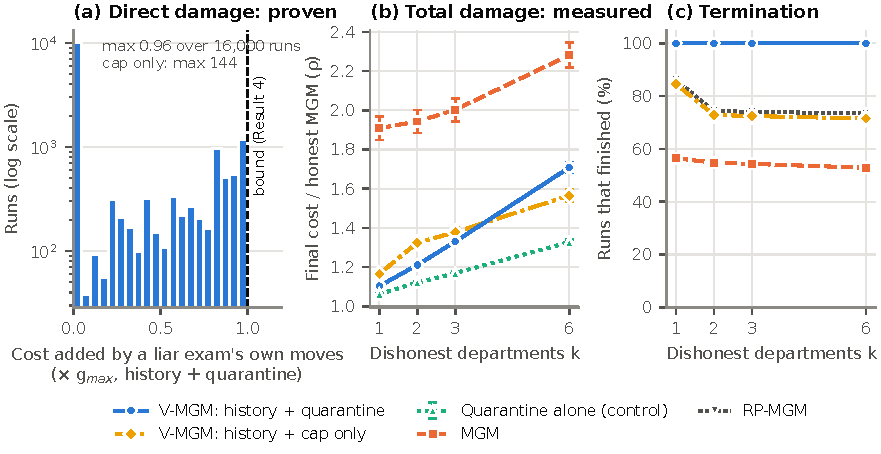
\includegraphics[width=\textwidth]{figures/fig1_guarantees.pdf}
\caption{The three guarantees, kept apart (E2, $k$ dishonest departments out of 12). (a) Direct damage, proven: the student cost added by a liar exam's own moves under history check + quarantine never reaches the bound of Result~\ref{res:bound}; with cap only it reaches $144\,\gmax$. (b) Total damage, measured: final cost relative to honest MGM grows with $k$; quarantining the same departments when nobody lies (control) accounts for most of it. (c) Termination: history check + quarantine finishes every run (Result~\ref{res:term}); MGM, RP-MGM and cap only do not, and a 1000-round limit does not help (E5). Error bars: 95\% CIs.}
\label{fig:guar}
\end{figure*}

\textbf{Several dishonest departments (RQ2, \Cref{fig:guar}, \Cref{tab:e2}).} With $k=1,2,3,6$ dishonest departments out of 12, placed next to each other or spread out, the history check flagged \emph{every} blocker and churner and never flagged an honest department. With quarantine, every run finished, while MGM finished 55\% and cap-only 75\% of runs under attack, and raising the round limit to 1000 changed none of them. The largest direct damage of any exam was $0.99\,\gmax$ over 58{,}440 runs. Total damage grows with $k$: $\rho=1.10, 1.21, 1.33, 1.71$ for $k=1,2,3,6$, against $1.91$--$2.28$ for MGM. The control shows that most of this is the cost of quarantine itself ($\rho=1.06$--$1.33$): a quarantined department's own preferences are ignored. Honest departments lose little beyond that (at most about 14 burden units more than under quarantine alone, at $k=6$). Placing liars next to each other made no significant difference.

\textbf{Quarantine vs cap only.} For selfish attacks (T1a, T2a), cap only already gives $\rho\approx1.00$ while quarantine costs about $0.33$; against churn, mixed attacks and sabotage, cap only fails ($\rho\approx1.7$--$2.3$, runs do not finish) and quarantine is needed (\Cref{tab:e2}, \Cref{fig:quar}). We keep quarantine because only it carries Results~\ref{res:term}--\ref{res:global}; a graded response (cap for oversized claims, quarantine for contradictions) is future work.

\begin{table}[t]
\centering
\footnotesize
\setlength{\tabcolsep}{4pt}
\caption{Mean $\rho$ with $k=3$ dishonest departments (E2; 400 runs per cell). $\dagger$: fewer than 95\% finished. ``Only'': nobody lies, the liars' departments quarantined from their flag rounds (control). Flagged: liars caught by history + quarantine (mixed: the third liar is a consistent saboteur).}
\label{tab:e2}
\begin{tabular}{lrrrrrrrr}
\toprule
Attack & MGM & RP-MGM & Hist.+cap & Hist.+quar. & Quar. only & Hist.+soft & Soft only & Flagged \\
\midrule
Block (T3a) & 4.43$^\dagger$ & 1.01 & 1.00 & 1.34 & 1.33 & 1.38 & 1.28 & 100\% \\
Churn (T3b) & 2.31$^\dagger$ & 1.36$^\dagger$ & 2.31$^\dagger$ & 1.36 & 1.29 & 1.37 & 1.17 & 99.9\% \\
Mixed attacks & 4.55$^\dagger$ & 1.30$^\dagger$ & 2.20$^\dagger$ & 1.39 & 1.21 & 1.43 & 1.16 & 67\% \\
Delayed contradiction (new) & 1.49$^\dagger$ & 1.02 & 1.01 & 1.35 & 1.10 & 1.38 & 1.04 & 81\% \\
Sabotage (T4) & 1.68$^\dagger$ & 1.74$^\dagger$ & 1.68$^\dagger$ & 1.57 & 1.06 & 1.57 & 1.03 & 75\% \\
Inflate huge (T2a) & 0.99 & 1.01 & 1.00 & 1.34 & 1.33 & 1.38 & 1.28 & 97\% \\
Exaggerate naive (T1a) & 0.98 & 1.01 & 1.00 & 1.33 & 1.33 & 1.37 & 1.25 & 87\% \\
Inflate in scale (T2b) & 1.00 & 1.01 & 1.00 & 1.03 & 1.05 & 1.04 & 1.03 & 32\% \\
Consistent sabotage (new) & 1.55 & 1.58 & 1.55 & 1.55 & 1.00 & 1.55 & 1.00 & 0\% \\
Exaggerate consistent (T1b) & 1.03 & 1.05 & 1.03 & 1.03 & 1.00 & 1.03 & 1.00 & 0\% \\
\bottomrule
\end{tabular}
\end{table}


\textbf{Lying vs algorithms (RQ1).} Blocking and churning raise MGM's cost by $3.6$ and $1.0$ over RP-MGM ($p<10^{-32}$); selfish inflation (T2) does no measurable harm, so H1 holds for malicious attacks only (\Cref{fig:h1}). RP-MGM and DSA ignore claims and so are not hurt by them, but they cannot name the liar, and RP-MGM still fails to finish under churn.

\textbf{Undetectable lying (RQ3).} No public check can flag a department that plays truthfully for stretched preferences $\lambda(g-\min g)$ (Result~\ref{res:undet}), and none was flagged. Its profit is near zero for $\kappa\le0.6$ and rises with $\kappa$ in every setting (Holm-corrected $p<0.05$), up to $+114$ at $\kappa=4.5$ (\Cref{fig:h3}). This only works when true preferences leave room on the scale; the pilot's T1b liar, which clips $\lambda g$ at $\gmax$, often loses.

\textbf{Problem size and neighbours (RQ4).} Because a liar's number of neighbours grows with $N$, we compare within each $N$ (\Cref{fig:h4}). Under MGM, blocking damage grows with the liar's neighbours at every $N$ (Spearman $+0.73$ to $+0.88$); churn and sabotage damage do not. Under V-MGM damage stays near zero at every degree, and with $N=48$ and 12 dishonest departments every run still finished.

%=====================================================================
\section{Limitations}
\label{sec:limits}
%=====================================================================
Checking needs shared-student counts and the timetable to be public (less privacy). Consistent lies stay undetected, and they pay once preferences are large relative to student costs (H3). Quarantine is what makes termination and the global bound hold, but it ignores the quarantined departments' own preferences, which is most of the remaining cost. Total cost relative to honest MGM is measured, not bounded, and Result~\ref{res:neg} shows it cannot be bounded. \textbf{Collusion} is out of scope: the checks and Results~\ref{res:hist}--\ref{res:global} work one department at a time, so the proven guarantees still hold when liars coordinate, but coordinated attacks could raise total damage, which we have not measured. Rooms and exam length are not modelled; random instances support comparisons, not real-timetable predictions.

%=====================================================================
\section{Contribution}
%=====================================================================
\vspace{-0.6em}
\begin{table}[H]
\centering\footnotesize
\begin{tabularx}{\linewidth}{@{}lX@{}}
\toprule
Member & Responsibilities \\
\midrule
Beli Dedhia & Problem model, attack model, proofs (Results 1--7); experiment design and statistics; report integration. \\
Khushi Garg & Instance generator and starting timetables; CP-SAT references; visualisation and demo. \\
Ananya Patel & MGM, RP-MGM and DSA implementations; pyDCOP validation; V-MGM checks and responses. \\
Poojan Soni & Attack strategies, including the undetectable ones; experiment runner, verification checks and plots. \\
All members & Literature review, writing and proofreading. \\
\bottomrule
\end{tabularx}
\end{table}
% TODO(team): update responsibilities to match who did what.

{\scriptsize\setlength{\bibsep}{0pt}\setlength{\columnsep}{12pt}
\begin{multicols}{2}
\bibliographystyle{unsrtnat}
\bibliography{references}
\end{multicols}}

%=====================================================================
\appendix
\section{Additional figures}
%=====================================================================
\begin{figure}[H]
\centering
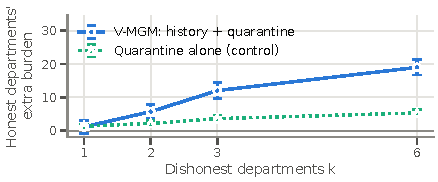
\includegraphics[width=\textwidth]{figures/fig2_quarantine_cost.pdf}
\caption{What quarantine costs, and who pays (E2). (a) By attack, $k=3$: cap only suffices for selfish attacks but fails for churn, mixed attacks and sabotage. (b) Honest departments' extra burden: most of the cost of quarantine falls on the quarantined departments.}
\label{fig:quar}
\end{figure}

\begin{figure}[H]
\centering
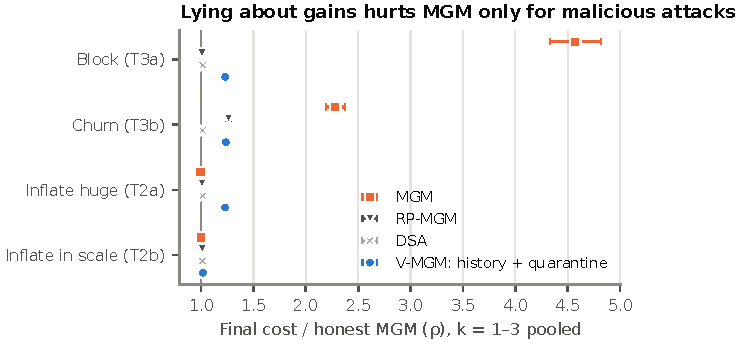
\includegraphics[width=0.6\textwidth]{figures/fig3_h1_algorithms.pdf}
\caption{Lying about gains hurts MGM only for malicious attacks (E1, $k=1$--$3$ pooled). Error bars: 95\% CIs.}
\label{fig:h1}
\end{figure}

\begin{figure}[H]
\centering
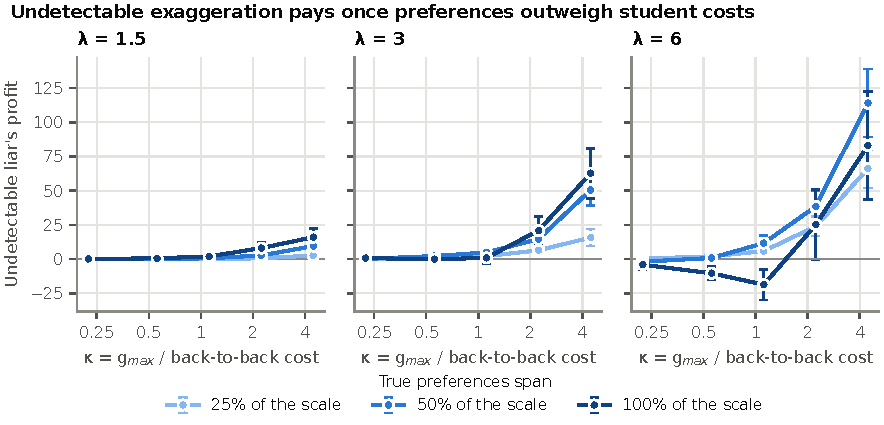
\includegraphics[width=\textwidth]{figures/fig4_h3_undetectable.pdf}
\caption{Profit of an undetectable liar (E3, $k=1$). It rises with $\kappa=\gmax/(W_s\bar n)$; true preferences that fill less of the scale leave more room to exaggerate.}
\label{fig:h3}
\end{figure}

\begin{figure}[H]
\centering
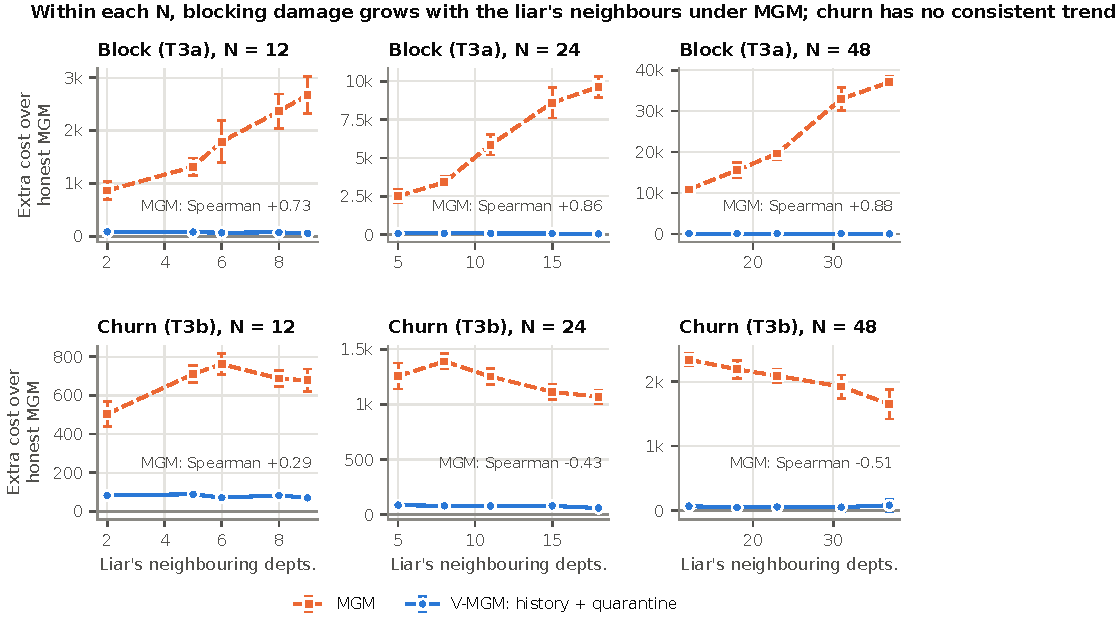
\includegraphics[width=\textwidth]{figures/fig5_h4_neighbours.pdf}
\caption{Damage against the liar's number of neighbours, separately for each $N$ (E4, $k=1$). Under MGM blocking damage grows with degree at every $N$; churn does not. Under V-MGM damage stays near zero.}
\label{fig:h4}
\end{figure}
\end{document}
